\documentclass{article}
\usepackage[utf8]{inputenc}
\usepackage{url}
\usepackage{hyperref}
\usepackage{draculatheme}
\usepackage{biblatex}
\usepackage{amsmath}
\usepackage{algorithm}
\usepackage{mathtools}
\usepackage{algpseudocode}
\usepackage{amsfonts}
\usepackage{IEEEtrantools}
\usepackage{parskip}
\usepackage{graphicx}
\usepackage[affil-it]{authblk}
\setlength{\abovecaptionskip}{0pt plus 3pt minus 0pt}
\addbibresource{mybib.bib}  

\title{\color{draculafg}\line(1,0){300}\\Modeling Neural Populations with Mixture Models\\\line(1,0){300}}
\author{\color{draculafg}Santiago M. Castro Dau}
\affil{Semester project for the Cortical Computation Group \\
	   Institute of Neuroinformatics,\\ University of Zürich and ETH Zürich}
\date{\color{draculafg}June 2022}

\begin{document}
\maketitle

\begin{abstract}
The central motivation for this work is to provide an alternative perspective on the
online K-means algorithm which is known to be analogous to a Winner takes it all
network. Furthermore we seek to improve said algorithm such that it becomes immune to the uneven
membership assignment problem, where occasionally and depending on
initialization one centroid is assigned responsibility over multiple
clusters of data points while others are left without any. 

We start by introducing Winner takes it all networks and their connection to the K-means algorithm. Then we introduce Mixture Models and show that the K-means algorithm can be seen as an instance of parameter
inference of a Gaussian Mixture Model. By showing this equivalence we point out a natural way to get rid of uneven
membership assignment. 

Then, using 
a Poisson Mixture Model we formulate an algorithm that we think is more fitting to represent neural populations and their dynamics. Finally we do some simulations and demonstrate the potential of the proposed algorithm. 

This work is very similar to \cite{Moraitis2021} and \cite{Keck2012} specially in terms of the theory
behind it, but the proposed algorithm differs from those proposed in
these papers. We argue that the framework used here and in the aforementioned papers provide a
probabilistic interpretation of the underlying learning process.

\end{abstract}

\pagebreak

\tableofcontents

\pagebreak

\section{Winner Take It All Networks}
Winner Takes it All Networks (WTAn) are a special kind of artificial neural network (ANN) for classification. They consist of two fully connected layers, the input and the output layer. 

\subsubsection*{Input layer}
We will refer to the \(i^{th}\) value associated with the \(i^{th}\) input neuron with \(x_i\), having in total \(M\) neurons in this layer. The entire input vector is denoted by \(\prescript{n}{}{x}\), where \(n\) denotes the index of the input, having in total \(N\) of these input vectors in one data set (Figure \ref{WTA}). 

\subsubsection*{Output layer}
Likewise we will refer to any of the \(K\) neurons in the output layer as neuron \(z_j\). The goal is to optimally classify the inputs using the \(K\) output neurons (Figure \ref{WTA}). 

\subsubsection*{Connections between layers}
Associated with every connection between any \(x_i\) and \(z_j\) neurons we have the weight \(\lambda_{ji}\). Every output neuron has a collection of weights associated to it denoted by \(\lambda_{j:}\). We use \(\Lambda\) to describe all of the weights in matrix from where \(\lambda_{j:}\)'s are the rows of the matrix (Figure \ref{WTA}). 

\begin{figure}[h]
    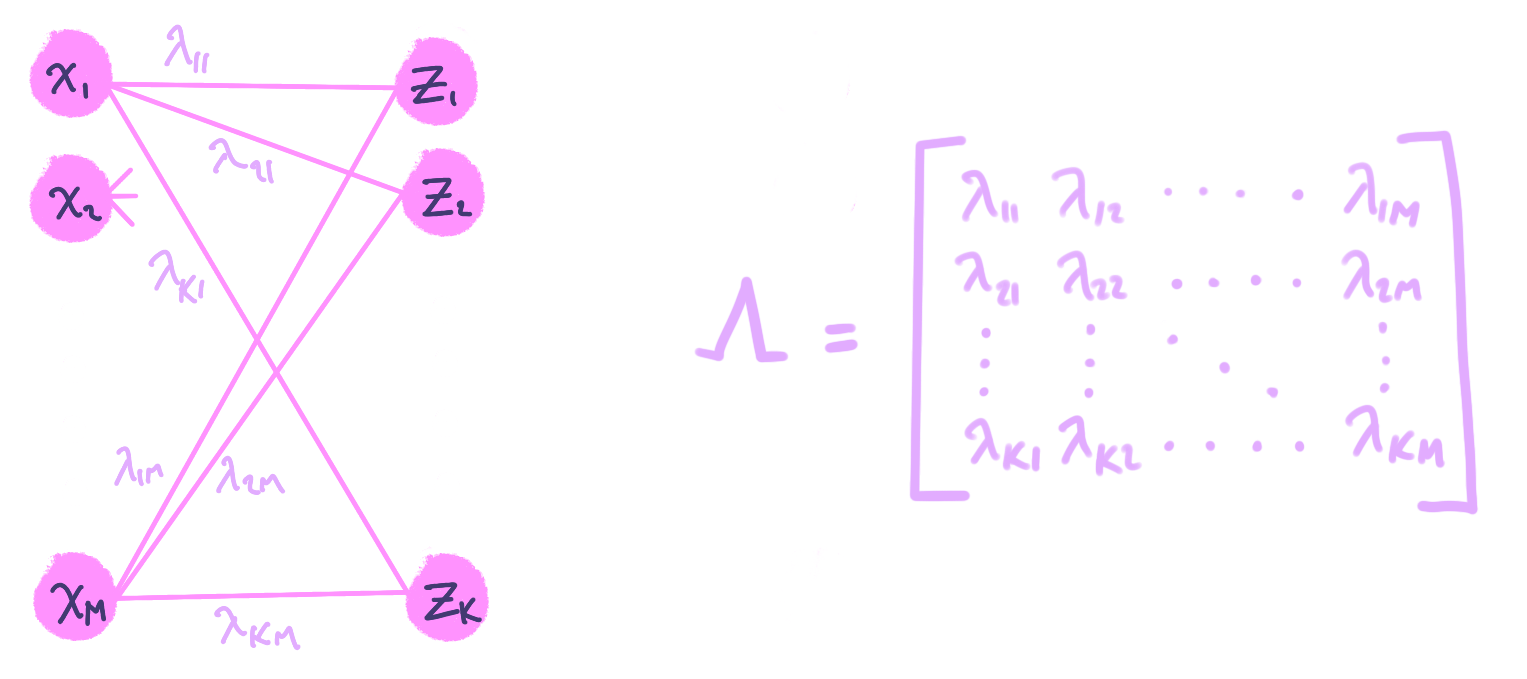
\includegraphics[width=\textwidth]{img/Untitled_Artwork.png}
    \caption{Schematic representation of the WTAn described in this section. \label{WTA}}
\end{figure}

WTAn have been studied in computational neuroscience because they provide a simple
model for a common connectivity pattern in the brain cortex, where
neurons compete with each other for activation through lateral
inhibition \cite{Keck2012}.

Lateral inhibition is modeled by making it so only one neuron is activated in the output layer per input. The winning neuron is the one with weights \(\lambda_{j:}\) that are the closest,
according to some measure of distance, to the \(n^{th}\) input vector
\(x\) \footnote{When its not important to indicate the index of the data point,
\(x\) will be used instead of \(\prescript{n}{}{x}\)}. It is important to note that in these networks the inputs do not get multiplied by the weights like in most ANNs, but are simply compared to the inputs on every iteration in order to find the closest \(\lambda_{j:}\). 

Learning takes place through adjustments of the weights every time an input is presented to the network (e.g in a n online fashion). The idea is that given an input pattern
\(\prescript{n}{}{x}\), the associated weights \(\lambda_{j:}\) of winning neuron
\(z_j\) get adjusted such that if the same or a similar input
\(^{n+1}x\) is presented to the network then \(z_j\) is again the
winner, thereby successfully classifying the input. 

Even thou it is convenient to think of all \(\lambda_{j:}\) weights
associated with winning neuron \(z_j\) to be updated as a whole in
vector form, we can also think of the update as taking place
individually for each element of \(\lambda_{ji}\), associated with input
neuron \(x_i\) and output neuron \(z_j\). The weight updates then become
akin to Hebbain learning where learning happens locally at each synapse.

If we restrict the weights and the inputs to be normalized, such that
the sum of the elements in the input vectors \(x\) and the weight vectors
\(\lambda_{j:}\) are equal to a constant \(\alpha\) \eqref{norm1} \eqref{norm2}, we can
implement the learning by nudging the previous weight vectors
\(\lambda_{j:}\) in the direction of the input. This nudge would be a function of the difference between
\(\lambda_{j:}\) and input vector \(x\) \eqref{km-nudge}. \footnote{For more
information on the biological plausibility and  of
normalization in biological neural circuits we refer the reader to \cite{Keck2012}.}

\begin{IEEEeqnarray}{rCl} 
\sum_{i=1}^M \lambda_{ji} &=& \alpha \label{norm1}\\
\sum_{i=1}^M x_i &=& \alpha \label{norm2} \\
\lambda^{(t)}_{j:} &\leftarrow& \lambda^{(t-1)}_{j:} - \eta \epsilon'(x - \lambda^{(t-1)}_{j:}) \label{km-nudge}
\end{IEEEeqnarray}

Here \(^{(t)}\) indicates the index of the iteration in the context of an
algorithm, and \(\eta\) is a small positive learning rate.

If we choose the squared L2 norm as our measure of distance
\(\epsilon(x - \lambda^{(t-1)}_{j:})\) we can take the derivative w.r.t
\(\lambda_{j:}\) and use the result as the update function
\(\epsilon'(x - \lambda^{(t-1)}_{j:})\) \eqref{l2norm} - \eqref{okm_nudge}.

\begin{IEEEeqnarray}{rCl} 
\epsilon(x - \lambda^{(t-1)}_{j:}) &=& \frac{1}{2} ||x - \lambda^{(t-1)}_{j:}||_2^2 \label{l2norm} \\
\frac{d}{d\lambda^{(t-1)}_{j:}} \epsilon(x - \lambda^{(t-1)}_{j:})  &=& \frac{d}{d\lambda^{(t-1)}_{j:}} \frac{1}{2} ||x - \lambda^{(t-1)}_{j:}||_2^2 \\
 &=& -(x - \lambda^{(t-1)}_{j:}) \\
 &=& \epsilon'(x - \lambda_{j:}) \\
 \lambda^{(t)}_{j:} & \leftarrow & \lambda^{(t-1)}_{j:} + \eta (x - \lambda^{(t-1)}_{j:}) \label{okm_nudge}
\end{IEEEeqnarray}

The result is an online version of the K-means algorithm (Algorithm \ref{online-kmeans}), where upon an input, the closest centroid (here the weights \(\lambda_{j:}\)) gets
pulled towards the coordinates of the input \(x\) \eqref{okm_nudge}. 

\begin{algorithm}
\caption{Online K-means} \label{online-kmeans}
\begin{algorithmic}
\State \textbf{Step 0.} Initialize parameters for each centroid.

$$
\Lambda \leftarrow \text{init.}
$$

\State \textbf{Step 1.} For every incoming $n$ data point find the closes cluster.

$$
\prescript{n}{}{z^{(t)}_j} = \underset{\lambda_{j:}}{\operatorname{arg min}} \| \prescript{n}{}{x} - \lambda_{j:}\|_2^2
$$

\State \textbf{Step 2.} Update the winning centroid $z_j$

$$
\lambda^{(t)}_{j:} \leftarrow \lambda^{(t-1)}_{j:} + \eta (x - \lambda^{(t-1)}_{j:})
$$

\State \textbf{Step 3.} Repeat step 1 and 2 for every incoming input

\end{algorithmic}
\end{algorithm}

A perfect
equivalence with the K-means algorithm would require that all the inputs
\(\prescript{n}{}{x}\) to be presented at once. In such case we would simply adjust our
cost function to account for all the data points \(N'\) associated to
the winning neuron \(z_j\). By minimizing this quantity, applying the
derivative, setting it to zero and solving for \(\lambda_{j:}\) \eqref{batch_1} - \eqref{batch_2}, we find
that the update is the same as in the K-means algorithm (Algorithm \ref{kmeans}), showing the
equivalence between these two seemingly different clustering schemes.

\begin{IEEEeqnarray}{rCl} 
\epsilon(X - \lambda_{j:}) &=& \frac{1}{2} \sum_{n=1}^{N'} ||\prescript{n}{}{x} - \lambda_{j:}||_2^2  \label{batch_1} \\
\hat{\lambda_{j:}} &=& \underset{\lambda_{j:}}{\operatorname{arg min}} \frac{1}{2}  \sum_{n=1}^{N'} ||\prescript{n}{}{x} - \lambda_{j:}||_2^2 \\
\hat{\lambda_{j:}} &=& \frac{1}{N'} \sum_{n=1}^{N'} (\prescript{n}{}{x}) \label{batch_2}
\end{IEEEeqnarray}

\begin{algorithm}
\caption{K-means} \label{kmeans}
\begin{algorithmic}
\State \textbf{Step 0.} Initialize parameters for each centroid.

$$
\Lambda \leftarrow \text{init.}
$$

\State \textbf{Step 1.} For all $N$ data points find the closes cluster and assign it
membership over the data point.

$$
\prescript{n}{}{z^{(t)}_j} = \underset{\lambda_{j:}}{\operatorname{arg min}} \| \prescript{n}{}{x} - \lambda_{j:}\|_2^2
$$

\State \textbf{Step 2.} Update the $K$ centroids, with the average of the coordinates of its
children data points.

$$
\lambda_{j:}^{(t+1)} = \frac{1}{N'} \sum_{n=1}^{N'} (\prescript{n}{}{x})
$$

\State \textbf{Step 3.} Repeat step 1 and 2 until convergence

\end{algorithmic}
\end{algorithm}

The vanilla WTAn as well as the K-means algorithm have the problem
that because only the weights \(\lambda_{j:}\) associated to the wining
neuron \(z_j\) get updated, it is common for some centorids to be
assigned two or more clusters of data points, while other centroids are
left without ``children'' data points and hence never get updated. Here
we call this issue uneven membership assignment (Figure \ref{uma}). 

\begin{figure}[h]
\centering 
    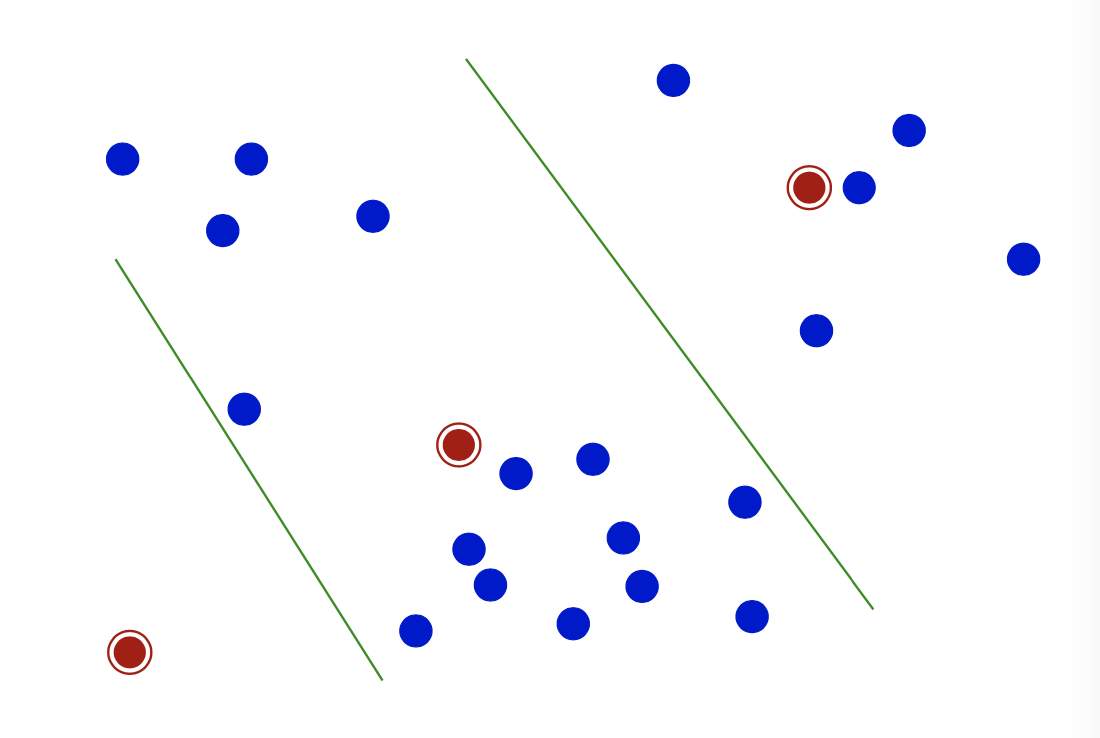
\includegraphics[width=0.5\textwidth]{img/problems_kmeans.png}
    \caption{Schematic representation uneven membership assignment. \label{uma}}
\end{figure}

This is partly due to the ``hardness'' of the assignment step, or in other words the fact that
only one neuron can win and therefore represent a given input. By
modeling centroids as being only partly responsible for a given data
point, instead of belonging exclusively to one, we can bypass
this problem. This idea of responsibility allows us to model multiple output neurons getting
activated upon an input, which is a more realistic model of the dynamics in a population of neurons. In order to formally define this notion of responsibility we must first introduce mixture models. 

\section{Mixture Models}
A mixture model is a probabilistic model for representing the presence
of sub populations within an overall population, without requiring that
an observed data set identifies the sub-population to which an
individual observation belongs (e.g without labels). Usually mixture models are used to make
statistical inferences about the properties of the sub-populations given
only observations on the pooled population \cite{Mixture_model}.

Just by reading this description we can already sense that mixture
models might be a good fit for modeling the classification of patterns as
in the WTAn, where we seek to differentiate between distinct input sub-populations. The idea is
that each observations is distributed according to a mixture of components, where all the components belong to the same parametric family of distributions but with different parameters \eqref{mm_likl}. The parameters of each component represent the distinct sub-populations and so we then seek to find the parameters that best explain our data in terms of some number of sub-populations. We specify a mixture model with he following notation (note the correspondence to the previous section).

\begin{itemize}
\item
  \(K\) is the number of mixture components, individual components indicated
  with subscript \(j\). Sometimes we refer to components as clusters, mixtures, sub-populations, and further on as output neurons. 
\item
  \(N\) is the number of observations, individual observations indicated with
  left superscript \(n\), where each observation
  $\prescript{n}{}{x} \in \mathbb{R}^M$ and \(\prescript{n}{}{x_i}\) is the \(i^{th}\)
  element of the \(n^{th}\) observation.
\item
  \(w\) is the vector of mixture weights
  where \(w_j\) is the mixture weight of component \(j\). Can also be
  expressed as the prior probability \(P(z_j|\theta)\) of a random data
  point belonging to any of the \(K\) components. Note that
  \(\sum_{j=1}^k w_j = 1\)
\item
  \(\Lambda\) is the matrix of parameters, where rows
  \(\lambda_{j:}\) are the parameters that correspond to the $j^{th}$ component.
  \(\lambda_{ji}\) denotes the the \(ji^{th}\) entree of $\Lambda$.
\item
  $\prescript{n}{}{z} \in \mathbb{R}^K$ is the vector of probabilities where \(\prescript{n}{}{z_j}\) is
  RV representing the probability of data point \(n\) belonging to
  cluster j.
\item
We will use $z_j$ without superscript as a marker variable indicating that we are referring only to the distribution of component $j$. For example $P(x | z_j , \theta)$. Indicates the probability that standpoint $x$ came from the distribution of component $j$.
\item
  $^{(t)}$ indicates the index of the iteration in the context of an algorithm.
\item
  \(\theta = \{w, \Lambda\}\) is the set of all parameters
\end{itemize}

The likelihood of one data point can be written as follows, where
\(P(x | z_j , \theta)\) is the probability density function of the
\(j^{th}\) component.

\begin{IEEEeqnarray}{rCl} 
\mathcal{L}(x:\theta) &=& \sum_{j=1}^K P(z_j|\theta) P(x | z_j , \theta) \label{mm_likl} \\
\mathcal{L}(x:\theta) &=& \sum_{j=1}^K w_j P(x | z_j , \theta)
\end{IEEEeqnarray}

There is two main inference problems when dealing with mixture models.
On one hand one would like to know the number and functional form
(parametric family) of the components within a mixture. This is usually
referred to as the system identification. On the other hand one would
like to estimate the corresponding parameter values given a fixed number
of components and their functional form. This is referred to as
parameter estimation \cite{Mixture_model}. In this work we concern ourselves with he problem of
parameter estimation, since we assume that the number of components and
their underlying distributions is fixed. Furthermore we take Expectation
Maximization as or method of choice for inference. \footnote{The reason behind this choice is that we
will show that a constrained form of EM for Gaussian Mixture Models is equivalent to K-means.}

In the context of mixture models, the EM can be seen as a unsupervised
learning algorithm. This is interesting because if it is applicable to
learning in WTAs it loosely implies that it might be useful to reason
about learning in the brain as an unsupervised learning procedure, where
the hidden RVs are the stimuli which generate specific input
pattern distributions (the observed RV) that the brain then categorizes
as belonging to the stimuli or cause by tuning the weights of the synapses.

\subsection{The EM algorithm}
After initialization of the parameters, the EM
starts by performing the expectation step (E-step)
followed by a maximization step (M-step) which completes one full
iteration. These two steps are repeated until the parameters converge.

In the E-step we seek to find the responsibility \(\gamma_j(\prescript{n}{}{x})\) of
each cluster on each data point \(\prescript{n}{}{x}\), or in other words the
probability that data point \(\prescript{n}{}{x}\) belongs to cluster \(j\).

\begin{IEEEeqnarray}{rCl} 
\gamma_j(\prescript{n}{}{x}) &=& P (z_j | \prescript{n}{}{x}, \theta) \\
&=& \frac{P(z_j, \prescript{n}{}{x}, \theta)}{P(\prescript{n}{}{x}, \theta)} \\
&=& \frac{P(\prescript{n}{}{x}|z_j, \theta) P(z_j | \theta)}{P(\prescript{n}{}{x}| \theta)}\\
P(\prescript{n}{}{x}|\theta) &=& \sum_k P(\prescript{n}{}{x}|\theta, z_k) P(z_k|\theta)
\end{IEEEeqnarray}

We know from before that \(P(z = j|\theta) = w_j\) are the prior
probabilities and \(P(\prescript{n}{}{x}|\theta, z = k)\) is the likelihood, which
depends on the parametric family we decide on.

\begin{IEEEeqnarray}{rCl} 
\gamma_j(\prescript{n}{}{x}) &=& \frac{w_jP(\prescript{n}{}{x}|\theta, z_k)}{\sum_{j=1}^K w_k P(\prescript{n}{}{x}|\theta, z_k)} \label{gamma}
\end{IEEEeqnarray}

Once we have all the \(\gamma\)'s for each data point, we have a
fully annotated data set, and can now move on to infer the parameters
\(\theta\) in the M-step using the previously estimated \(\gamma\)'s. For
this we take the expression of the likelihood of the data given the
parameters and we maximize its lower bound. The derivation is as
follows.

We can rewrite equation \eqref{gamma} accounting for all
\(N\) data points, applying the log and then Jensen's inequality to get
the lower bound on the data likelihood \footnote{For a more detailed derivation
we refer the reader \cite{malone_2014}.}. We maximize this
quantity \eqref{b_theta} instead of the log likelihood directly simply because of the log likelihood is hard to evaluate.

\begin{IEEEeqnarray}{rCl} 
\mathcal{\log L}(D:\theta) &\ge & b(\theta)\\
\mathcal{\log L}(D:\theta) &=& \sum_{n=1}^N\log\sum_{j=1}^K w_j P(\prescript{n}{}{x} | z_j , \theta) \\
b(\theta) &=& \sum_{n=1}^N \sum_{j=1}^K \gamma_j(\prescript{n}{}{x})\log\frac{w_j P(\prescript{n}{}{x} | z_j , \theta)}{\gamma_j(\prescript{n}{}{x})} \label{b_theta}
\end{IEEEeqnarray}

We can then expand the logarithm, distribute \(\gamma_j(\prescript{n}{}{x})\), and
split the sum.

\begin{IEEEeqnarray}{rCl} 
b(\theta) &=& \sum_{n=1}^N \sum_{j=1}^K \gamma_j(\prescript{n}{}{x})\log w_j P(\prescript{n}{}{x} | z_j , \theta) - \sum_{n=1}^N \sum_{j=1}^K \gamma_j(\prescript{n}{}{x})\log \gamma_j(\prescript{n}{}{x})
\end{IEEEeqnarray}

Because the \(\gamma_j(\prescript{n}{}{x})\)'s are already fixed from the E-step we can
concentrate only on the first term which we term \(Q(\theta)\).

\begin{IEEEeqnarray}{rCl} 
Q(\theta) &=& \sum_{n=1}^N \sum_{j=1}^K \gamma_j(\prescript{n}{}{x})\log w_j P(\prescript{n}{}{x} | z_j , \theta)
\end{IEEEeqnarray}

To get an estimate for the parameters \(\theta\) we perform the
partial derivatives with respect to each individual parameter (e.g. \(\lambda_{ji}\) and \(w_j\)),
make it equal to 0, and solve for the corresponding parameter. This will
look different depending on the parametric family we choose and also the
assumptions we make (e.g if we uniform fixed priors or we have them
fixed).

\begin{algorithm}
\caption{EM algorithm} \label{generic_em}
\begin{algorithmic}
\State \textbf{Step 0.} Initialize parameters.
$$
\theta \leftarrow \text{init.}
$$

\State \textbf{E-step.} Compute $\gamma_j(\prescript{n}{}{x})$ for each \(n\) data point and each component \(j\).
$$
\gamma_j(\prescript{n}{}{x}) = \frac{w_jP(\prescript{n}{}{x}|\theta, z_j)}{\sum_{j=1}^K w_k P(\prescript{n}{}{x}|\theta, z_j)}
$$

\State \textbf{M-step.} Optimize the lower bound of the log likelihood $Q(\theta)$ to update $\theta$.
$$
\frac{dQ(\theta)}{d \theta} = \frac{d}{d \theta}\sum_{n=1}^N \sum_{j=1}^K \gamma_j(\prescript{n}{}{x})\log w_j P(\prescript{n}{}{x} | z_j , \theta)
$$

\State \textbf{Step 3.} Repeat E and M-step until \(\theta\) converges.
\end{algorithmic}
\end{algorithm}

\subsection{Gaussian Mixture Models}
In the following subsection we show that by considering the components of a mixture
model to be Gaussian and by further constraining it, namely by enforcing
fixed spherical variances in all components and fixed uniform mixture weights, we
recover the K-means algorithm, which implies that we might be able to
use the EM algorithm to device a more general procedure for learning
with a WTAn. This constrained version of the EM algorithm is termed
the Hard EM for Gaussian Mixture Models (GMMs). We start by deriving the unconstrained version of the EM which yields a
similar version of K-means but with soft membership assignment, which
naturally eases the uneven membership problem. This is called the Soft
EM for GMMsGMMs.

% TODO: left here 

\subsubsection{The Soft EM for GMMs}
We simply have to plug in our Gaussian assumption, e.g. $P( \prescript{n}{}{x} | \theta, z_j) = \mathcal{N}(\prescript{n}{}{x}|\theta, z_j)$. The parameters then become $\theta = \{w, \mu, \Sigma\}$, where each component $j$ has its own collection of parameters $\{w_j, \mu_j, \Sigma_j\}$ \footnote{Note that we assume each component to be multivariate Gaussian}. 

\begin{algorithm}
\caption{Soft EM for GMMs} \label{soft_em}
\begin{algorithmic}
\State \textbf{Step 0.} Initialize parameters $\theta = \{w, \mu, \Sigma\}$.
$$
\theta \leftarrow \text{init.}
$$

\State \textbf{E-step.} Compute $\gamma_j(\prescript{n}{}{x})$ for each \(n\) data point and each component \(j\).
$$
\gamma_j(\prescript{n}{}{x}) = \frac{w_j\mathcal{N}(\prescript{n}{}{x}|\theta, z_j)}{\sum_{j=1}^K w_k \mathcal{N}(\prescript{n}{}{x}|\theta, z_k)}
$$

\State \textbf{M-step.} Update $\theta$.
\[
w_j^{(t)} \leftarrow \frac{1}{N'} \sum_{i=1}^{N'} \gamma_j^{(t)}(\prescript{n}{}{x}) 
\]

\[
\mu_j^{(t)} \leftarrow \frac{\sum_{i=1}^{N'} \gamma_j^{(t)}(\prescript{n}{}{x})\prescript{n}{}{x}}{\sum_{i=1}^{N'} \gamma_j^{(t)}(\prescript{n}{}{x})}
\]

\[
\Sigma_j^{(t)} \leftarrow \frac{\sum_{i=1}^{N'} \gamma_j^{(t)}(\prescript{n}{}{x})(\prescript{n}{}{x}-\mu_j^{(t)})(\prescript{n}{}{x}-\mu_j^{(t)})^T}{\sum_{i=1}^{N'} \gamma_j^{(t)}(\prescript{n}{}{x})}
\]

\State \textbf{Step 3.} Repeat E and M-step until \(\theta\) converges.
\end{algorithmic}
\end{algorithm}

\subsubsection{The Hard EM for GMMs}

For the Hard EM the E-step classifies each data point as belonging to
only one of the clusters. Intuitively we choose the cluster with the highest $P (z_j | \prescript{n}{}{x}, \theta)$, then we make $\gamma_j(\prescript{n}{}{x}) = 1$ for all but the wining component, and 0 for the rest. Then by enforcing fixed
spherical variance in all components ($\Sigma_1,...,\Sigma_K = I\sigma$) and fixed uniform mixture weights ($\forall j, w_j = \frac{1}{K}$), we are only left with the updates of $\mu_j$ that simplify into the simple average of all the data points belonging to cluster $j$.

We can also simplify the E-step as follows. As stated above we seek the cluster that maximizes $P (z_j | \prescript{n}{}{x}, \theta)$.

\begin{IEEEeqnarray}{rCl} 
\prescript{n}{}{z^{(t)}} = \underset{j}{\operatorname{arg max}} P(z_j | \prescript{n}{}{x}, \theta^{(t-1)})
\end{IEEEeqnarray}

We can decompose \(P(z_j | \prescript{n}{}{x}, \theta^{(t-1)})\) using Bayes rule to
get the follwoing expression.


\begin{IEEEeqnarray}{rCl} 
\prescript{n}{}{z^{(t)}} = \underset{j}{\operatorname{arg max}} \frac{1}{Z} P(z_j | \theta^{(t-1)}) P(\prescript{n}{}{x} | z_j, \theta^{(t-1)}) 
\end{IEEEeqnarray}

\(\frac{1}{Z}\) is the normalization constant from Bayes rule which is
also independent of \(z\) and therefor can be omitted in the maximization. By assuming that each cluster has the same size, \(P(z | \theta^{(t-1)})\) to be constant we can take them out of the maximization argument.

\begin{IEEEeqnarray}{rCl} 
\prescript{n}{}{z^{(t)}} = \underset{j}{\operatorname{arg max}} \frac{1}{\sqrt{(2\pi\sigma^2)^d}} \exp(\frac{-1}{2\sigma^2} \| \prescript{n}{}{x} - \mu_j^{(t-1)}\|_2^2 )
\end{IEEEeqnarray}

We can see again that the maximization is only over the squared 2-norm
and we can also note that maximizing this quantity is equivalent to
minimizing the 2-norm.

\begin{IEEEeqnarray}{rCl} 
\prescript{n}{}{z^{(t)}} = \underset{z}{\operatorname{arg min}} \| \prescript{n}{}{x} - \mu_j^{(t-1)} \|_2
\end{IEEEeqnarray}

Thereby the E-step becomes to Step 1 of K-means (Algorithm \ref{kmeans}). 

\begin{algorithm}
\caption{Hard EM for GMMs} \label{hard_em}
\begin{algorithmic}
\State \textbf{Step 0.} Initialize parameters $\theta = \mu$.
$$
\mu \leftarrow \text{init.}
$$

\State \textbf{E-step.} Compute $\prescript{n}{}{z^{(t)}}$ for each \(n\) data point.
$$
\prescript{n}{}{z^{(t)}} = \underset{z}{\operatorname{arg min}} \| \prescript{n}{}{x} - \mu_j^{(t-1)} \|_2
$$

\State \textbf{M-step.} Update $\mu$.
$$
\mu_j^{(t)} = \frac{1}{N'} \sum_{n=1}^{N'} (\prescript{n}{}{x})
$$

\State \textbf{Step 3.} Repeat E and M-step until \(\theta\) converges.
\end{algorithmic}
\end{algorithm}

We can now see that by considering constant variances and
weights the Hard EM (Algorithm \ref{hard_em}) performs exactly the same operations as the K-means (Algorithm \ref{kmeans}) and is therefore equivalent.

By relaxing both the constant variances and
weights constraint we allow the underlying cluster to have
different sizes and elliptical shapes, which allowed us to capture richer structures in the data. Doing so often leads to enhanced performance specially when the clusters are overlapping. 

Likewise, by
using membership instead of hard assignments we account for the
uncertainty of the assignments. This help poorly initialized clusters get updated, since
even if they are far away from data points initially, they will still have a
responsibility over them and will therefore move towards the data. Thus this approach resolves the uneven membership assignment issue that is encountered in K-means and vanilla WTAn.

\section{Optimization Via Gradient Accent}
The EM formulated above updates the parameters by performing MLE over $N$ data points. Because this involves a group of data points and we would like an algorithm that updates the parameters base only on one observations at a time (e.g. online), we turn towards gradient accent. By continuously take small steps in the direction of the gradient of the lower bound of the likelihood function $Q(\theta)$, one can eventually reach a local maximum of $Q(\theta)$ \cite{piech_2018}. 

In the following we show this approach for the Gaussian and constrained Hard EM. 

\begin{IEEEeqnarray}{rCl} 
\mu_j^{(t)} &=& \mu_j^{(t-1)} + \eta \frac{\delta Q(\mu_j^{(t-1)})}{\delta \mu_j^{(t-1)}} \label{ga} \\
Q(\theta) &=& \sum_{n=1}^N \sum_{j=1}^K \gamma_j(\prescript{n}{}{x})\log w_j P(\prescript{n}{}{x} | z_j , \theta)
\end{IEEEeqnarray}

Since in the Hard EM all \(\gamma_j(\prescript{n}{}{x})\) are 0 except for that the
parent component, the variance is spherical, and we only have one data point
(\(N = 1\)) we have that \(Q(\theta)\) is equal to:

\begin{IEEEeqnarray}{rCl} 
Q(\theta) &=& \log P(x | z_j , \theta) = \log w_j \mathcal{N}(x | z_j , \mu_j, \Sigma_j)\\
&=& \log w_j + \log \frac{1}{\sqrt{(2\pi\sigma^2)^d}} + \log \exp(\frac{-1}{2\sigma^2} \| x - \mu_j^{(t-1)}\|_2^2 )
\end{IEEEeqnarray}

We can further remove positive constant multipliers because they don't affect the direction of the gradient and terms that don't include \(\mu_j^{(t-1)}\), because they will be 0 anyway when we take the derivative. 

\begin{IEEEeqnarray}{rCl} 
Q(\theta) &=&  -\| x - \mu_j^{(t-1)}\|_2^2 \\
\frac{\delta Q(\mu_j^{(t-1)})}{\delta \mu_j^{(t-1)}} &=& 2 ( x - \mu_j^{(t-1)}) 
\end{IEEEeqnarray}

We can again remove the 2 because it does not affect the direction of the gradient. Plugging in this into equation \eqref{ga} we obtain the following. 

\begin{IEEEeqnarray}{rCl} 
\mu_j^{(t)} = \mu_j^{(t-1)} + \eta' ( x - \mu_j^{(t-1)}) 
\end{IEEEeqnarray}

We see how this recovers the online K-means algorithm shown in the first
section (Algorithm \ref{online-kmeans}). Now that we have a way of deriving an update rule we can go back to a general mixture model, decide on the parametric family and derive and EM algorithm that can also be computed with a modified WTAn. Specifically we will choose this family to be the Poisson distribution. 

\section{EM for Poisson Mixture Models}
Previously we chose the likelihood of the data \(P(x | z, \theta)\) to
be Gaussian but this was simply to show the equivalence with the K-means
algorithm. It might make more sense to use the Poisson since we
would can think of entrees in \(\prescript{n}{}{x_i}\) vectors to represent spiking events. This makes
sense since a Poisson RV represents the number of occurrences or a random
event withing a specific time frame. Furthermore, with normal distributions
there is always a possibility that a number drawn from such distribution
is negative which would not make sense if we decide to think of the inputs as spiking events.

\subsection{E-step}

\begin{equation*}
\gamma_j(\prescript{n}{}{x}) = P (z_j | \prescript{n}{}{x}, \theta) = \frac{P(\prescript{n}{}{x}|z_j, \theta) P(z_j | \theta)}{\sum_k P(\prescript{n}{}{x}|\theta, z_k) P(z_k|\theta)} \tag{\ref{gamma} revisited}
\end{equation*}

\(P(\prescript{n}{}{x}|\theta, z_j) = \prod_{i=1}^M \text{Pois}(\prescript{n}{}{x_i}; \lambda_{ji})\),
where \(\lambda_{ji}\) denotes the rate parameter of component \(j\)
from element \(i\) of the \(n^{th}\) input. Note that this assumes that
that the input from each neuron is generated form an independent
Poisson, when in reality there might be strong correlation between the
activities \(x_i\). Here we limit ourselves to the independent case but perhaps there is a more fitting way of expressing
this likelihood, maybe as a multivariate Poisson \cite{inouye2017}.

\begin{IEEEeqnarray}{rCl}
\text{Pois}(\prescript{n}{}{x_i}; \lambda_{ji}) &=& Pr(X=\prescript{n}{}{x_i}) = \frac{\lambda_{ji}^{\prescript{n}{}{x_i}} e^{-\lambda_{ji}}}{\prescript{n}{}{x_i}!}\\
\gamma_j(\prescript{n}{}{x}) &=& \frac{w_j \prod_{i=1}^M \text{Pois}(\prescript{n}{}{x_i}; \lambda_{ji})}{\sum_{k=1}^K w_k \prod_{i=1}^M \text{Pois}(\prescript{n}{}{x_i}; \lambda_{ki})}\\
 &=& \frac{w_j \exp{\bigg(\sum_{i=1}^M \prescript{n}{}{x_i}\log\lambda_{ji}} \bigg)}{\sum_{k=1}^K w_k \exp{\bigg(\sum_{i=1}^M \prescript{n}{}{x_i}\log\lambda_{ki}\bigg)}} \label{softmax}\\
 &=& \frac{w_j \prod_{i=1}^M \lambda_{ji}^{\prescript{n}{}{x_i}} }{\sum_{k=1}^K w_k \prod_{i=1}^M \lambda_{ki}^{\prescript{n}{}{x_i}} }
\end{IEEEeqnarray}

\subsection{M-step}

\begin{IEEEeqnarray}{rCl}
Q(\theta) &=& \sum_{n=1}^N \sum_{j=1}^K \gamma_j(\prescript{n}{}{x})\log w_j P(\prescript{n}{}{x} | z_j , \theta)\\
&=& \sum_{n=1}^N \sum_{j=1}^K \gamma_j(\prescript{n}{}{x_i})\log w_j \prod_{i=1}^M \frac{\lambda_{ji}^{\prescript{n}{}{x_i}} e^{-\lambda_{ji}}}{\prescript{n}{}{x_i}!}\\
&=& \sum_{n=1}^N \sum_{j=1}^K \gamma_j(\prescript{n}{}{x}) \bigg( \log w_j + \sum_{i=1}^M \log \frac{\lambda_{ji}^{\prescript{n}{}{x_i}} e^{-\lambda_{ji}}}{\prescript{n}{}{x_i}!}\bigg)
\end{IEEEeqnarray}

The derivative of every term which does not involve the \(\lambda_{ji}\)
is 0, thus we can ignore such terms.

\begin{IEEEeqnarray}{rCl}
\frac{\delta Q(\theta)}{\delta \lambda_{ji}} &=& \frac{\delta}{\delta \lambda_{ji}} \sum_{n=1}^N \gamma_j(\prescript{n}{}{x}) \bigg( \log w_j + \log \lambda_{ji}^{\prescript{n}{}{x_i}} + \log e^{-\lambda_{ji}} - \log(\prescript{n}{}{x_i}!)\bigg)\\
&=& \frac{\delta}{\delta \lambda_{ji}} \sum_{n=1}^N \gamma_j(\prescript{n}{}{x}) \bigg( \log w_j + {\prescript{n}{}{x_i}} \log \lambda_{ji} -\lambda_{ji} - \log(\prescript{n}{}{x_i}!)\bigg)\\
&=& \sum_{n=1}^N \gamma_j(\prescript{n}{}{x}) \bigg( \frac{\prescript{n}{}{x_i}}{\lambda_{ji}} - 1\bigg)
\end{IEEEeqnarray}

For the batch case the closed form MLE estimate for the new
\(\lambda_{ji}\) and \(w_j\) are as follows.

\begin{IEEEeqnarray}{rCl}
\lambda_{ji} &=& \frac{\sum_{n=1}^{N} \gamma_j(\prescript{n}{}{x_i}) \prescript{n}{}{x_i}}{\sum_{n=1}^{N} \gamma_j(\prescript{n}{}{x_i})}\\
w_j &=& \frac{\sum_{n=1}^{N} \gamma_j(\prescript{n}{}{x_i})}{N}
\end{IEEEeqnarray}

Furthermore we can consider the update via gradient ascent in which case
we get the following expressions.

\begin{IEEEeqnarray}{rCl}
\lambda_{ji}^{(t)} &\leftarrow & \lambda_{ji}^{(t-1)} + \eta \frac{\delta Q(\theta)}{\delta \lambda_{ji}}\\
\lambda_{ji}^{(t)} &\leftarrow & \lambda_{ji}^{(t-1)} + \eta \gamma_j(\prescript{n}{}{x}) \bigg( \frac{\prescript{n}{}{x_i} - \lambda_{ji}^{(t-1)}}{\lambda_{ji}^{(t-1)}} \bigg) \label{lr}
\end{IEEEeqnarray}

If we consider the \(w_j\)'s to be fixed we need only update the
centroids \(\lambda_{ji}\). Note that in this case we kept the constant
positive multiplier \(\gamma_j(\prescript{n}{}{x})\) since it provides a way to modulate
the strength of the learning depending on the degree of responsibility
that the mixture \(j\) over element \(i\) of data point \(n\).

\begin{algorithm}
\caption{Online EM for a PMM} \label{pois_em}
\begin{algorithmic}
\State \textbf{Step 0.} Initialize parameters.
$$
\Lambda \leftarrow \text{init.}
$$

\State \textbf{E step.} Compute $\gamma_j(\prescript{n}{}{x})$ for each \(n\) data point and each component \(j\).
$$
\gamma_j(\prescript{n}{}{x}) = \frac{w_j \exp{\bigg(\sum_{i=1}^M \prescript{n}{}{x_i}\log\lambda_{ji}} \bigg)}{\sum_{k=1}^K w_k \exp{\bigg(\sum_{i=1}^M \prescript{n}{}{x_i}\log\lambda_{ki}\bigg)}}
$$

\State \textbf{M-step.} Optimize the lower bound of the log likelihood $Q(\theta)$ to update $\Lambda$.
$$
\lambda_{ji}^{(t)} \leftarrow  \lambda_{ji}^{(t-1)} + \eta \gamma_j(\prescript{n}{}{x}) \bigg( \frac{\prescript{n}{}{x_i} - \lambda_{ji}^{(t-1)}}{\lambda_{ji}^{(t-1)}} \bigg)
$$

\State \textbf{Step 3.} Repeat E and M step at every input.

\end{algorithmic}
\end{algorithm}


Its not difficult to see that the Online EM for a PMM (Algorithm \ref{pois_em}) is not too different from the online K-means (Algorithm \ref{online-kmeans}). Instead of neurons in the output layer having all or non responses we have a normalized output $\gamma_j(\prescript{n}{}{x})$ as a weighted soft-max function \eqref{softmax}. This is a different and perhaps more accurate way of modeling the response of a population to an input, specially when considering lateral inhibition. The learning rule is again not too different, the only difference being that the change in the coefficient is the ratio of the difference and the old parameter, scaled by the normalized output $\gamma_j(\prescript{n}{}{x})$ \eqref{lr}. In sum, we propose this modified version of the WTAn with the operations described in algorithm \ref{soft_em}.

\section{Discussion}
By showing that a WTAn is equivalent to an online
version of the EM algorithm we also show that it shares the same
theoretical assurances, namely that algorithm maximizes the lower bound
of the likelihood. But perhaps even more importantly, it gives us a
probabilistic framework which we can use to reason about the learning.

Specifically, the mixture weights \(w_j = P(z_j | \theta)\) can be
thought of as the overall probability that a random data point belongs
to any given component. Here we propose that such probability can be
seen as the homeostatic neuronal activity of the output neurons,
e.g. the probability that a neuron will get activated, regardless of the
input. While our model does not learn these parameters, we set them
a priori as hyper-parameters.

Furthermore \(\gamma_j(\prescript{n}{}{x}) = P (z_j | \prescript{n}{}{x}, \theta)\) can be view as the
same probability but conditional on the input or alternatively, the
percentage of activity that output neuron \(j\) has relative to all of
the output neurons. In a biological context it would be natural that the
intensity with which the output neuron reacts to a stimuli affects the
strength of the learning, that is the magnitude of the change in the
synaptic weights \eqref{lr}. 

It would also makes sense
that the mixing weights \(w_j\) are taken into account for the
computation \(\gamma_j(\prescript{n}{}{x})\), the relative activation of output neuron
\(j\) (note that the mixing weights are only present in the computation
of the \(\gamma_j(\prescript{n}{}{x})\)).

Naturally this normalized activity \(\gamma_j(\prescript{n}{}{x})\) is where the
lateral inhibition of the output neurons is modeled, such that the overall
activity is a function of the activity of all of the neurons in the
output layer. This division operation could be implemented approximately
with shunting inhibition of example, where the other neurons in the
output layer set the conductance such that the gain and the summation
dynamics of neuron \(z_j\) are is determined by the activity of all
other neurons \cite{carandini1994}. This is due to the fact
that the output voltage of a postsynaptioc neuron can be modeled as
being inversely proportional to the conductance (set by lateral shunting
inhibition) and directly proportional to the driving current resulting
from the temporal and spatial summation of inhibitory and expiatory
inputs coming from the input layer. Alternative ways of activity
normalization have been proposed including synaptic scaling and
feed-forward inhibition \cite{carandini2012} \cite{pouille2009}. It is not
clear how exactly a ensemble of biological neurons would implement exactly the
operation to compute \(\gamma_j(\prescript{n}{}{x})\).

We further note that the proposed algorithm consists only of computing
the normalized output of each neuron and then updating the synaptic
weights, which as you can see from equation \eqref{lr}
only involves the quantities that are local to the synapse, and is thus quite
Habbian like. 

Perhaps a word of caution since it does not make
sense to think of $\lambda_{ji}$ as synaptic weights, but rather as the rate at which neuron $i$ fires at neuron $j$,
where each neuron $j$ can have a different guess for the rate $\lambda_{ji}$ \footnote{Perhaps there is away to show that the synaptic weights is somehow connected to parameter \(\lambda_{ji}\).}. 
When both $\lambda_{ji}$ and $x_i$ are big, the more neuron $j$ will get activated, and when there is a discrepancy between these two, the $\lambda_{ji}$ will be pushed around to match the input.

In the following section we provide the results from the simulations of the proposed algorithm. The code in this available in this \href{https://github.com/Sann5/neural_populations}{\color{draculacyan} gitHub repository}. 

\section{Simulations}
\subsection{Simulations specifications}
We tested out algorithm on the MNIST data-set \cite{deng2012mnist}. We adjusted the weights through 30 epochs of the training split and tested the performance of the classification on the testing split. Since every image is $28$ by $28$ pixels the input dimension (number of nodes in the input layer) is $784$ and we chose the output dimension to be 50 in order to capture heterogeneity across digits. 

Each training and testing image was normalized, and scaled in compliance with equations \eqref{norm1} and \eqref{norm2}. After we summed 1 to every pixel to avoid numerical problems. We chose the previously mentioned scaling factor $\alpha = 784$, but since we added 1 to every pixel the overall intensity in every image came out to be $1568$, which was the scaling factor we used for the Lambdas.  

The \(\lambda_{ji}\) were initialized according to the mean pixel value across the processed training split plus its standard deviation weighted by numbered drawn from a uniform random distribution. Finally the images were flattened to a 1-dimensional tensor to facilitate matrix operations. 

The simulations were run in two scenarios, uniform fixed mixing weights and log-normal. The sections below shows the results for the uniform mixing weight scenario and we discuss the impact of changing the mixing weights in a subsequent subsection. 

For more implementation details please see the \href{https://github.com/Sann5/neural_populations}{\color{draculacyan} simulations code}.

\subsection{Evolution of the $\lambda_{ji}$}
In figure \ref{gen_filed_evo} we can see the evolution of the \(\lambda_{j:}\) in heatmap form after each one of the 30 epoch, starting from the top left and going to the right before going down to the next row. 

\begin{figure}[h]
    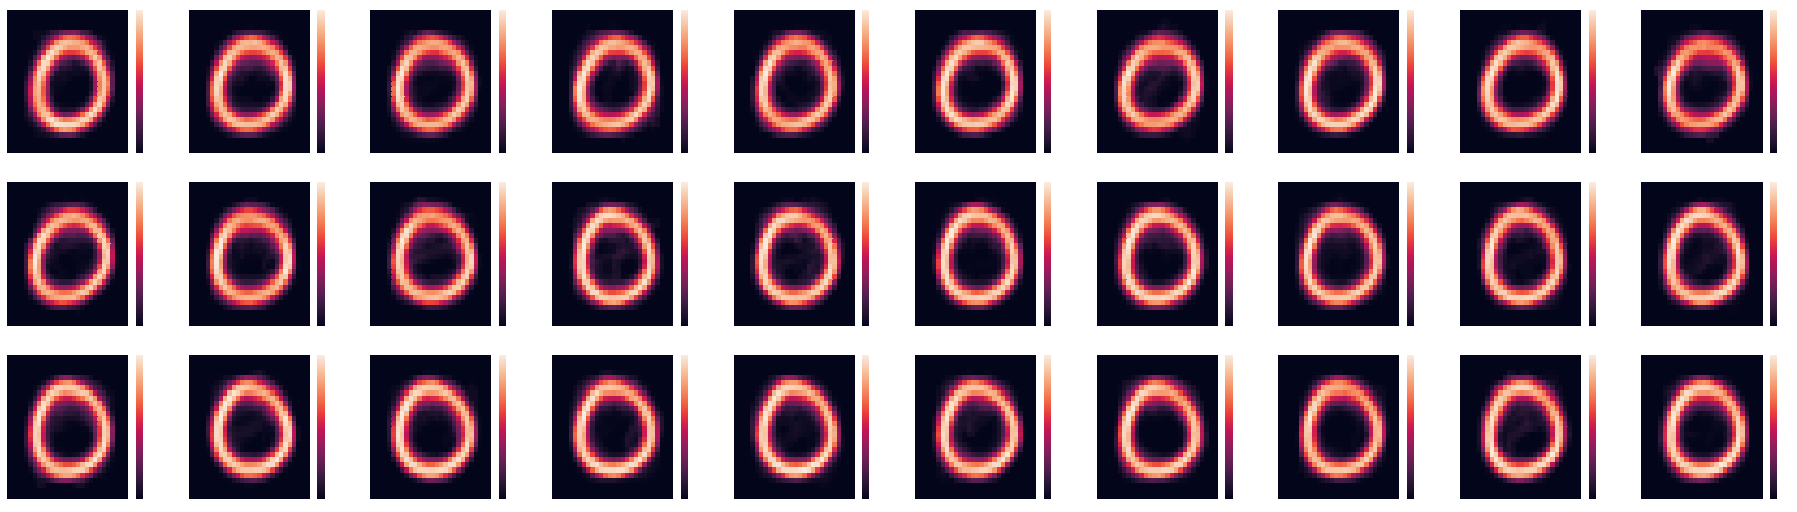
\includegraphics[width=\textwidth]{img/output_41_1.png}
    \caption{Heatmaps of the generative field of the first neuron after each of the 30 epochs. \label{gen_filed_evo}}
\end{figure}

The first this that caches the eye is that individual neurons display a generative field that resembles a digit. This is a nice result as it indicates that each neuron is the steward of a generative field corresponding to one of the 10 classes. These results are in agreement with the results in \cite{Keck2012}.

The second one is that perhaps 30 epochs is an over kill since it seems that already after the first one the \(\lambda_{j:}\) have settled down into one of the digits. In the next figure you can see the generative fields for each one of the 50 neurons after 30 epochs of training.

\begin{figure}[h]
    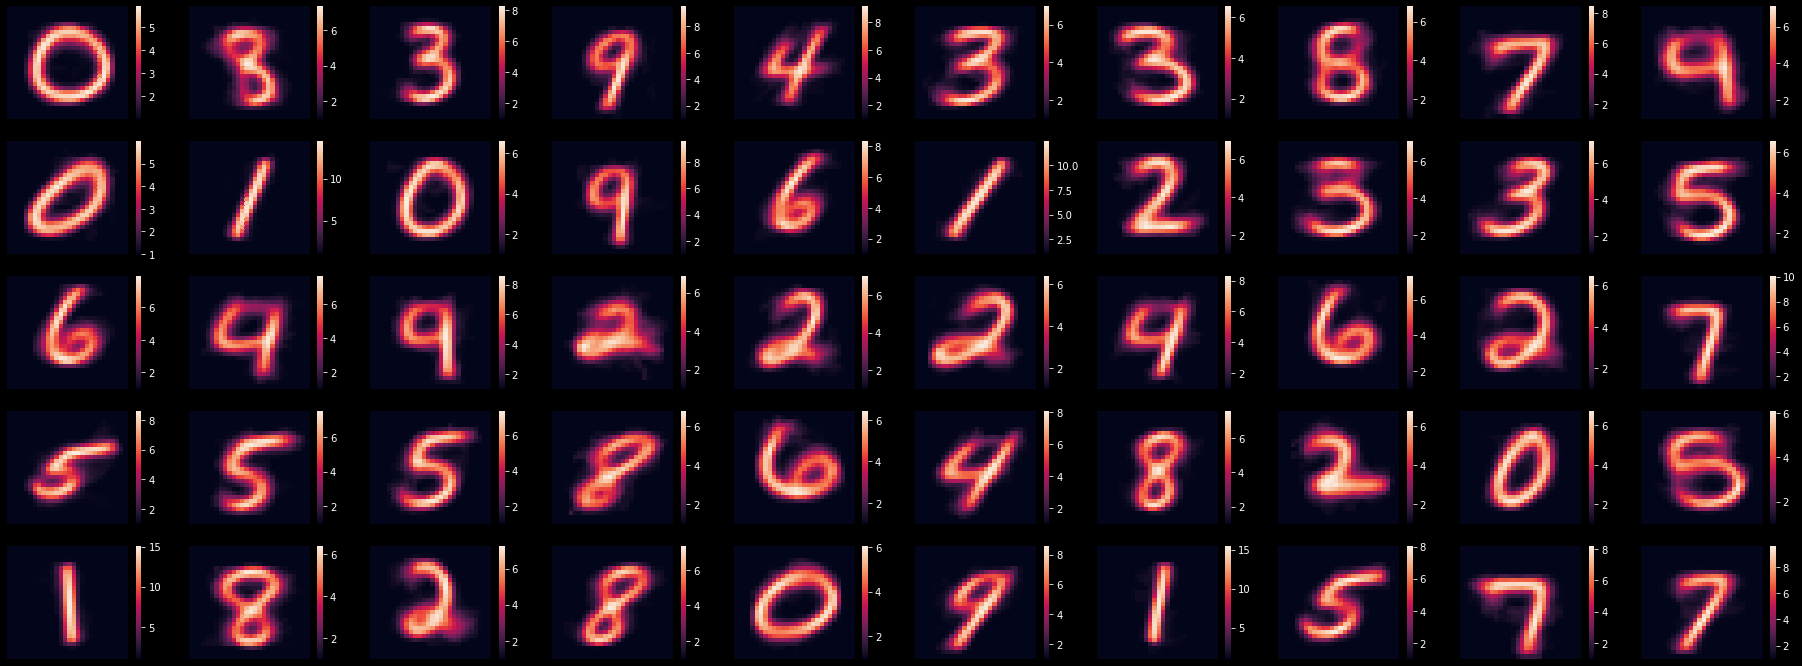
\includegraphics[width=\textwidth]{img/output_43_1.png}
    \caption{Heatmaps of the generative field of all neurons after 30 epochs. \label{gen_fileds}}
\end{figure}

We can see that there are multiple neurons representing one single digit, which perhaps helps capture heterogeneity in the typography. For the following classification performance analysis we manually annotated each one of the neurons according to the digit they display in their generative field. 

\subsection{Classification Performance}
The next figure show the the performance of the trained algorithm in predicting the correct class of the testing images. For each image we computed the \(\gamma_j(\prescript{n}{}{x})\) vector, and counted as on-probability the value of the \(\gamma_j(\prescript{n}{}{x})\)'s that corresponded to the label of the input, and off-probability the  \(\gamma_j(\prescript{n}{}{x})\) of all the other neurons. We summed these on and off probabilities for each neuron for the whole testing split. Then we aggregated all of the on-probability mass for neurons representing the same digit and the same for the off mass. This quantities are then represented in the bar char below.

\begin{figure}[h]
    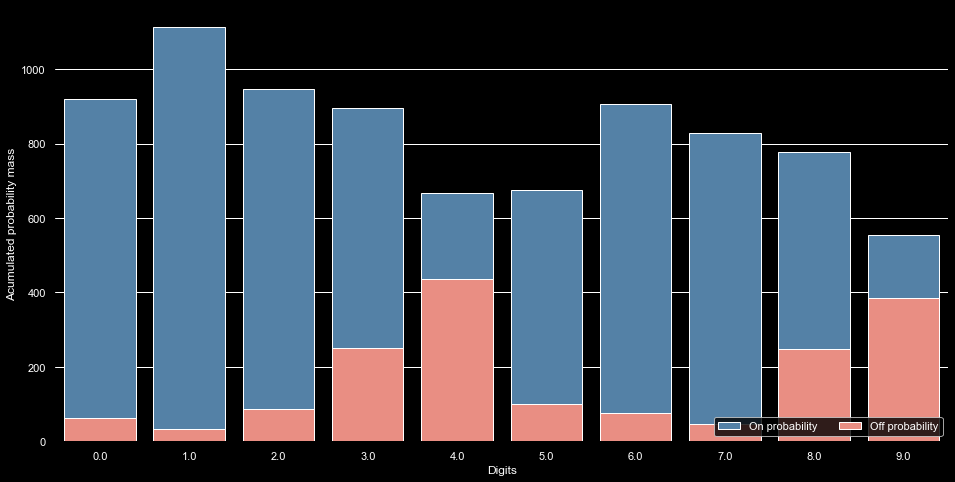
\includegraphics[width=\textwidth]{img/output_47_0.png}
    \caption{Off and on probability of predictions for every image on the testing split. \label{on-off}}
\end{figure}

We can see that there is a significant amount of off-probability specially for digits 4 and 9 which are often very similar. In fact when you look at the number of images that are classified correctly according to the maximally exited neuron, only around 80\% of the test images classified correctly. 

To further investigate why the performance is not better even when the generative fields show neat digits we displayed examples where the input was not classified correctly along with the top 10 maximal exited neurons (Figure \ref{ts}). It seems that because the \(\gamma_j(\prescript{n}{}{x})\) only care about overlap between the generative field and the input there can be miss classifications when the input overlaps more with a different digit. 

\pagebreak

\texttt{Label of input:  4\\}
\texttt{Heatmap of input image:\\}
\begin{figure}[!h]
    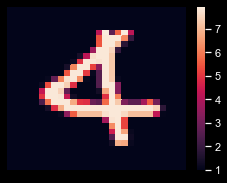
\includegraphics[scale=0.3]{img/output_51_1.png}
\end{figure}

\texttt{Probability of image belonging to the first 10 components:}

\texttt{[1.0000e+00, 8.4539e-23, 1.7772e-23, 3.1410e-32, 1.1038e-33,\\ 
		3.9651e-46, 3.0196e-49, 4.7079e-61, 4.6908e-64, 5.2946e-66]}

\texttt{Top 10 generative fields:}
\begin{figure}[h]
    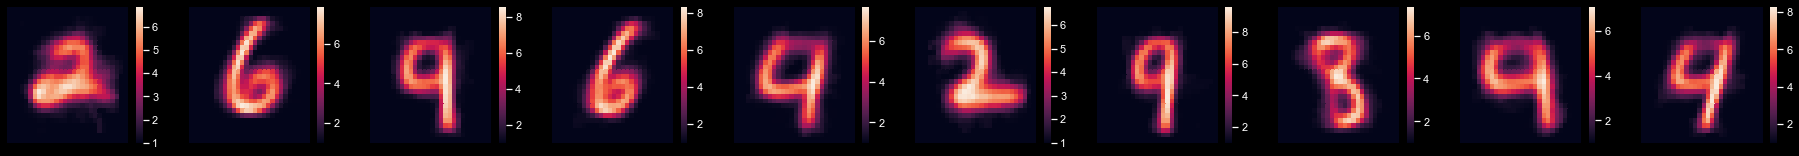
\includegraphics[width=\textwidth]{img/output_51_4.png}
    \caption{Display of code showing the top 10 generative fields for a miss classified image. \label{ts}}
\end{figure}\\

We can also note that the probabilities for all subsequent neurons are usually quite low with the maximal \(\gamma_j(\prescript{n}{}{x})\) often approximating 1. This might be a numerical issue that needs further investigation. Ideally we would like our network to faithfully represent uncertainty in the input, spreading more evenly the probability mass along the output neurons. 

\subsection{Effect of the Mixing Weights on Classification Performance}
The performance is very similar, perhaps slightly lower but would need further instigation \footnote{There is more variation in the performance between different runs of the simulations that variation between the uniform weights and log normal weights.}. Likewise there is the evolution of the weights and the resulting generative fields are very similar to the ones with the simulations where the mixing weights were uniform (images not shown).

\subsection{Future Perspectives}
In relation to the simulations and the theoretical framework presented before we present a list of further improvements to this work.

\begin{itemize}
\item
	The weights need not be kept constant, they could be updated just as the $\lambda_{ji}$'s. We hypothesize that specially when there is a large class imbalance, updating the mixing weights would have a strong impact on performance.  
\item 
	We can view the mixing weights as representing the prior on the class size, perhaps the algorithm learns to compensate for class imbalance by grouping together output neurons that share the similar generative fields. However weather this is actually happening in our simulations is jet to be investigated. 
\item
	As mentioned before the uncertainty in the prediction is not very well represented. Achieving an accurate representation would be a great way to improve performance. 
\item
	It would be interesting to explore whether one could perform more complex downstream tasks other than classification using this framework. One example of such task would the the addition of two numbers, where the input layer contains digits that come from two distinct underlying distributions and the output layer somehow represents the result of the sum. 
\item
	It would also be interesting to explore the implications of assuming a mixture model for the data to begin with with.
\item
	Finally the independence assumption for the derivation of the E-step in the Poisson EM can also have a large impact on performance but also on model complexity. 
\end{itemize}

\pagebreak
\printbibliography
\end{document}
